\documentclass[tikz, border=5mm]{standalone}
\usetikzlibrary{calc, positioning}
\usepackage{textcomp}
\tikzset{
% every node/.style={
% rectangle,
% draw,
% minimum width=2cm,
% minimum height=1.5cm
% },
% >=latex,
}

\begin{document}
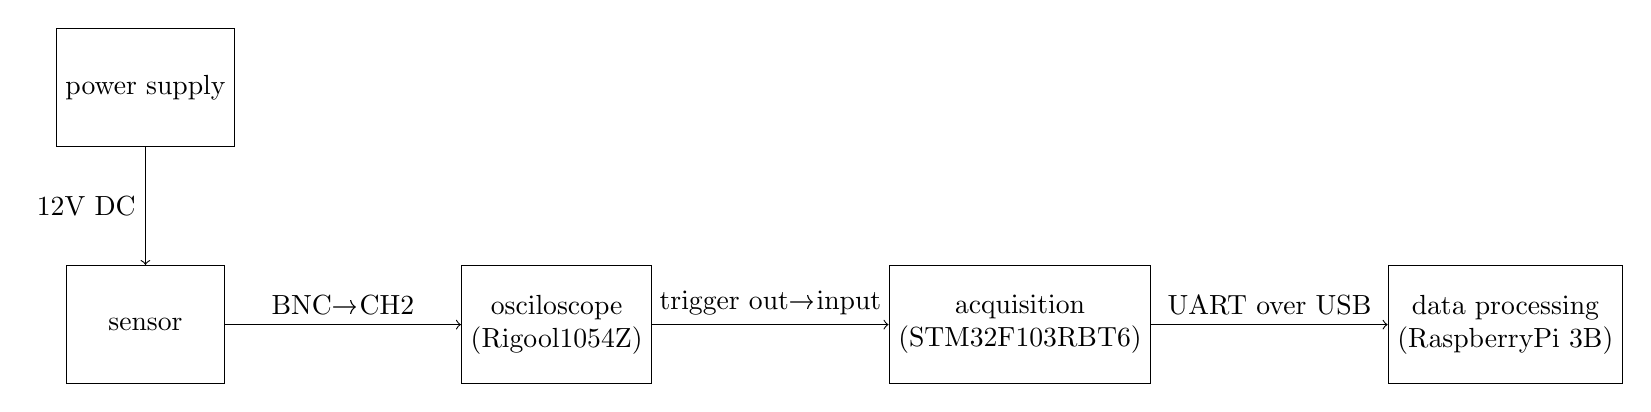
\begin{tikzpicture}[node distance=1.5cm and 3cm]
% Nodes
\node (one) [align=center, draw, minimum width=2cm, minimum height=1.5cm] {sensor};
\node (a0) [above=of one, align=center, draw, minimum width=2cm, minimum height=1.5cm] {power supply};
\node (a1) [right=of one, align=center, draw, minimum width=2cm, minimum height=1.5cm] {osciloscope\\ (Rigool1054Z)};
\node (a2) [right=of a1, align=center, draw, minimum width=2cm, minimum height=1.5cm] {acquisition\\ (STM32F103RBT6)};
\node (a3) [right=of a2, align=center, draw, minimum width=2cm, minimum height=1.5cm] {data processing\\ (RaspberryPi 3B)};

% Connectors
\begin{scope}[->]

%\draw[->] (one) -- +(20pt,0) node[a1] {$\mu$};

% \draw[->] (one) to node[pos=0.1,above, font=\small,above]{BNC} node [font=\small,above] {} to node[pos=0.1,above, font=\small,above]{BNC}(a1);

\draw [->] (a0) -- node[anchor=east, minimum width=.25cm, draw=none] {12V DC} (one);
\draw [->] (one) -- node[anchor=south, minimum height=.25cm, draw=none] {BNC\textrightarrow CH2} (a1);
\draw [->] (a1) -- node[anchor=south, minimum height=.25cm, draw=none] {trigger out\textrightarrow input} (a2);
\draw [->] (a2) -- node[anchor=south, minimum height=.25cm, draw=none] {UART over USB} (a3);

\end{scope}

\end{tikzpicture}
\end{document}